\chapter{Aplikacja do rozpoznawania gestów}
Projekt zakładał utworzenie aplikacji do rozpoznawania gestów w czasie rzeczywistym. Aplikacja została zaimplementowana za pomocą środowiska Visual Studio 2015 tworząc projekt WPF. Jak opisano w podrozdziale \ref{sec: WPF}, WPF to silnik graficzny do tworzenia aplikacji okienkowych, gdzie odpowiednie graficzne elementy oraz widoki są konstruowane za pomocą języka znaczników XAML. Język C\# posłużył do implementacji \textit{back-end'u} aplikacji, wykorzystano również elementy biblioteki Accord .NET, w skład których należały m.in. funkcje do obsługi kamery oraz filtracji obrazu, algorytm SURF jak również klasyfikator SVM. Dla części widocznej ze strony użytkownika zastosowano zestaw narzędzi o nazwie \textit{MahApps.Metro}, który nadpisuje domyślny styl graficznych elementów w silniku WPF.

\begin{figure}[h]
	\centering
	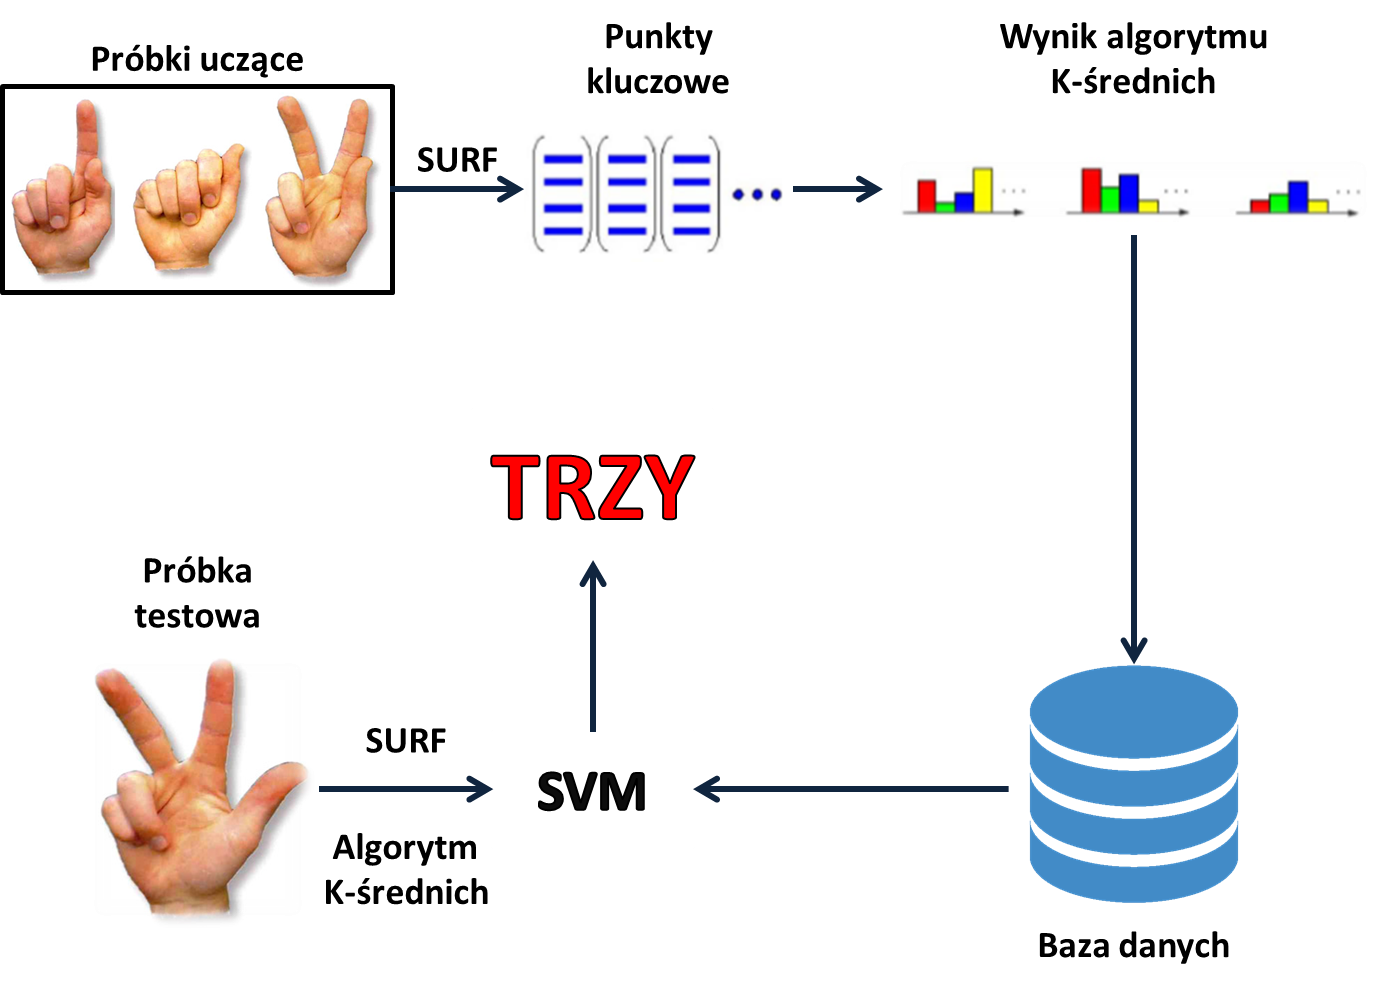
\includegraphics[width=16cm]{ApplicationFlowChart}
	\centering
	\caption{Schemat działania aplikacji.}
	\label{im: ApplicationFlowChart}
\end{figure}

Zasada działania aplikacji została przedstawiona na rysunku \ref{im: ApplicationFlowChart}. Próbki treningowe wraz z odpowiednimi etykietami są poddawane działaniu algorytmu SURF. Wynik operacji to zbiór punktów kluczowych dla każdego z obrazów. Następnie dokonywane jest grupowanie odpowiednich punktów w znaną z góry liczbę klastrów. Wyniki grupowania lądują w bazie danych, która jest wykorzystywana do utworzenia modelu SVM. 
Próbka testowa poddawana jest takim samym operacjom co wszystkie próbki uczące - jest ona przekształcana za pomocą algorytmu SURF oraz K-średnich w wektor o znanej liczbie klastrów. Model SVM klasyfikuje próbkę do jednej z podanych kategorii. 


W dalszej części rozdziału przedstawiono szczegółową implementację aplikacji. Pierwszy podrozdział zawiera opis wykorzystanych wzorców projektowych. W kolejnych podrozdziałach opisano każdy z widoków dostępnych w aplikacji wraz ze wzajemnymi zależnościami pomiędzy nimi.

\section{Wzorzec MVVM}
Wzorzec MVVM (skrót od ang. Model-View-ViewModel) jest jednym z wzorców architektonicznych służący do tworzenia oprogramowania. Daje możliwość pełnej separacji interfejsu użytkownika od modelu aplikacji. Twórcami wzorca są architekci firmy \textit{Microsoft} Ken Cooper oraz Ted Peters, którzy pracowali nad sposobem usprawnienia programowania sterowanego zdarzeniami. Wzorzec ten stał się jednym z komponentów nowo powstałego silnika graficznego WPF. 
W skład wzorca MVVM wchodzą następujące elementy:
\begin{itemize}
	\item Model: Reprezentuje prawdziwą zawartość aplikacji lub stanowi warstwę dostępu do danych.
	\item View (widok): jest to struktura, którą użytkownik widzi na ekranie swojego monitora.
	\item ViewModel: abstrakcyjna warstwa dla widoku udostępniająca publiczne własności oraz komendy. Za pomocą techniki \textit{data binding} widok wymienia informację z powiązanym z nim ViewModelem. ViewModel odpytuje model w celu pobrania lub zmiany danych. Zastosowanie struktury ViewModelu eliminuje istnienie bezpośredniego połączania pomiędzy widokiem a modelem.
\end{itemize}

\section{Wzorzec Mediator}


\section{Widoki aplikacji}
W niniejszej sekcji przedstawiono dokładny opis wszystkich okien wchodzących w skład aplikacji.
\subsection{Główny widok aplikacji}
NA rysunku RYSUNEK przedstawiono widok główny aplikacji do rozpoznawania gestów. W jego skład wchodzą następujące elementy:
\begin{itemize}
	\item 
\end{itemize}